\subsection{Dalil Sinus dan Dalil Cosinus}
    Misalkan $ABC$ adalah suatu segitiga dengan $R$ adalah panjang jari-jari lingkaran luarnya.
\begin{center}
    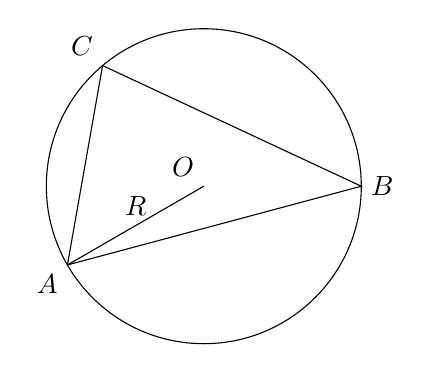
\begin{tikzpicture}
    \coordinate (O) at (0,0);
    \coordinate (B) at (0:2cm);
    \coordinate (A) at (210:2cm);
    \coordinate (C) at (130:2cm);
    
    \draw (O) circle (2cm);
    \draw (A) -- (B) -- (C) -- cycle;
    \node[right] at (B) {$B$};
    \node[below left] at (A) {$A$};
    \node[above left] at (C) {$C$};
    \node[above left] at (O) {$O$};
    \draw (A) -- node[above]{$R$} (O);
    \end{tikzpicture}
\end{center}
    \subsubsection{Dalil Sinus}
    $$\dfrac{BC}{\sin \angle A} = \dfrac{CA}{\sin \angle B}= \dfrac{AB}{\sin \angle C} = 2R$$
    
    \subsubsection{Dalil Cosinus}
    \begin{align*}
        AB^2 &= BC^2 + CA^2 - 2\cdot BC \cdot CA \cdot \cos \angle C\\
        BC^2 &= CA^2 + AB^2 - 2\cdot CA \cdot AB \cdot \cos \angle A\\
        CA^2 &= AB^2 + BC^2 - 2\cdot AB \cdot BC \cdot \cos \angle B
    \end{align*}

\subsection{Latihan Soal Dalil Sinus dan Cosinus}
\begin{enumerate}
    \item (OSK 2016) Pada segitiga $ABC$, titik $M$ terletak pada $BC$ sehingga $AB=7, AM=3, BM=5$, dan $MC=6$. Panjang $AC$ adalah \dots

    \item (OSK 2013) Misalkan $P$ adalah titik interior dalam daerah segitiga $ABC$ sehingga besar $\angle PAB = 10^\circ, \angle PBA = 20^\circ, \angle PCA = 30^\circ, \angle PAC=40^\circ$. Besar $\angle ABC = \dots$
    
    \item (Modifikasi OSK 2017) Pada sebuah lingkaran dengan pusat $O$, talibusur $AB$ berjarak 5 dari titik $O$ dan talibusur $AC$ berjarak $5\sqrt{2}$ dari titik $O$ dengan titik $A$ terletak di busur $BC$ yang lebih kecil ($A$ diantara $B$ dan $C$) Jika panjang jari-jari lingkaran 10, maka $BC^2=\dots$
\end{enumerate}